\documentclass[12pt,a4paper]{article}
\usepackage[utf8]{inputenc}
\usepackage[T1]{fontenc}
\usepackage[ngerman]{babel}
\usepackage{csquotes}
\usepackage[backend=biber,style=authoryear,maxcitenames=2,maxbibnames=99]{biblatex}
\addbibresource{Organisation.bib} % Bib-Datei nicht vergessen!
\newcommand{\zitat}[1]{\parencite{#1}}
\bibliography{Organisation}
\usepackage{geometry}
\geometry{
	left=30mm,
	right=30mm,
	top=25mm,
	bottom=25mm
}
\usepackage{graphicx}
\usepackage{float}
\usepackage{setspace}
\onehalfspacing
\usepackage{caption}
\usepackage{tocloft}
\usepackage{hyperref}
\hypersetup{colorlinks=true, linkcolor=black, urlcolor=blue, citecolor=black}
\usepackage{acronym}
\usepackage[nottoc]{tocbibind}
\usepackage{etoolbox} % für robusten Befehl
\usepackage{lipsum} % nur für Blindtext, kann entfernt werden
\usepackage{setspace} % für Zeilenabstand
\usepackage{ragged2e} % für \justifying


\newcommand{\absatzZitat}[1]{%
	\begin{quote}
		\fontsize{10pt}{12pt}\selectfont
		\setstretch{1.0}
		\leftskip=1cm
		\rightskip=1cm
		\justifying
		#1
	\end{quote}
}

\begin{document}
	
	%------------------------- Titelseite -------------------------
	\begin{titlepage}
		\centering
		\vfill
		{\Huge \textbf{Deutsche Telekom}}\\[1.5cm]
		\large
		Seminar: Grundlagen der Organisation\\
		Sommersemester 2025\\[2cm]
		
\includegraphics[width=0.4\textwidth]{images/UOL-Logo.png}\\[2cm]
		\normalsize
		\begin{flushleft}
			\textbf{Betreurin:} Prof. Dr. Julia Brennecke\\[0.5cm]
			\textbf{Abgegeben von:}\\
			Mika Scheinig\\
			Elija Wendte\\
			Justus Kressmann\\
			Engin Fidansoy\\
			Manar Krenbeh\\[0.5cm]
			Carl von Ossietzky Universität Oldenburg\\
			Fakultät II – Informatik, Wirtschafts- und Rechtswissenschaften\\
		\end{flushleft}
		\vfill
		\begin{flushright}
			Abgabedatum: 01. Juni 2025
		\end{flushright}
	\end{titlepage}
	
	%------------------------- Eidesstattliche Erklärung -------------------------
	\pagenumbering{Roman}
	
	\section*{\texorpdfstring{Executive Summary}{Executive Summary }}\label{executive-summary}
	
	In diesem Bericht wird die Aufbau- und Ablauforganisation der Deutschen
	Telekom AG untersucht, die mit rund 200.000 Mitarbeitenden in mehr als
	50 Ländern zu den größten Telekommunikationsanbietern weltweit gehört.
	Der Konzern organisiert sich im Wesentlichen divisional, wobei
	Matrixelemente in Bereichen wie IT, Personal und Strategie hinzukommen.
	Diese hybride Struktur soll Spezialisierung, Kund:innennähe und
	Flexibilität ermöglichen. Allerdings ergeben sich dabei auch
	Schwierigkeiten bei Koordination, Abstimmung und der Bestimmung
	eindeutiger Zuständigkeiten. Die Analyse legt offen, dass interne
	Abläufe teils als schwerfällig wahrgenommen werden.
	Entscheidungsprozesse nehmen viel Zeit in Anspruch, interdisziplinäre
	Kooperation funktioniert nicht optimal, und Silo-Denken erschwert eine
	übergreifende Sichtweise. Agile Arbeitsformen lassen sich unter diesen
	Bedingungen schwer integrieren. Bestehende Initiativen wie digitale
	Lernplattformen, neue Führungsmodelle und bereichsübergreifende Projekte
	sind wichtige Schritte, reichen jedoch nicht aus, um strukturelle
	Schwächen zu beheben.
	
	\noindent Der Schwerpunkt liegt auf der Geschäftseinheit T-Systems, bei der ein
	gesteigerter Veränderungsbedarf festgestellt wurde. Die Analyse zeigt
	Potenziale in Effizienz, Zuständigkeiten und Kulturentwicklung. Erste
	Handlungsideen wie klare Schnittstellen, effizientere Prozesse und
	vernetzte Zusammenarbeit werden skizziert. Der Bericht bildet die Basis
	für einen Folgebericht mit konkreten Empfehlungen zur Reorganisation von
	T-Systems.
	
	
	%------------------------- Inhaltsverzeichnis -------------------------
	\newpage
	\tableofcontents
	\newpage
	
	%------------------------- Abbildungsverzeichnis -------------------------
	\listoffigures
	\newpage
	
	%------------------------- Tabellenverzeichnis -------------------------
	\listoftables
	\newpage
	
	%------------------------- Abkürzungsverzeichnis -------------------------
	\section*{Abkürzungsverzeichnis}
	\begin{acronym}[IT]
		\acro{IT}{Informationstechnologie}
		\acro{BWL}{Betriebswirtschaftslehre}
	\end{acronym}
	\newpage
	
	%------------------------- Kapitelstruktur -------------------------
	
	\pagenumbering{arabic}
	\setcounter{page}{1}
	\begin{center}
		\textbf{Report 1 – Deutsche Telekom}
	\end{center}
	
	
	
	\section{Einleitung und Unternehmensvorstellung}
	
	Angesichts einer wirtschaftlichen Umgebung, die aufgrund von
	Unsicherheit, technologischer Dynamik und steigender Komplexität geprägt
	ist, müssen Unternehmen heute besonders anpassungsfähig sein. Wegen des
	digitalen Wandels, neuer Arbeitsformen, wachsender Kund:innenerwartungen
	sowie Herausforderungen wie demografischem Wandel und Fachkräftemangel
	müssen bestehende Strukturen und Prozesse regelmäßig überprüft werden.
	\zitat{kornmeier2022} Oft ist es nicht mehr ausreichend, bestehende
	Strukturen nur geringfügig anzupassen. Es bedarf einer grundlegenden
	Reflexion über die Struktur- und Prozessorganisation. Insbesondere in
	großen Unternehmen mit internationalen Geschäftstätigkeiten sind
	entscheidende Fragen zu beantworten: Wie rasch ist es möglich,
	Entscheidungen zu treffen? Sind die Zuständigkeiten klar zugeteilt? Wie
	gut arbeitet die Koordination zwischen den vielen organisatorischen
	Einheiten?
	
	\noindent Die in Bonn ansässige Deutsche Telekom AG zählt zu den größten
	
	\noindent Telekommunikationsunternehmen der Welt. Der Konzern operiert in mehr als
	50 Ländern, hat rund 200.000 Angestellte und erwirtschaftete im Jahr
	2023 einen Umsatz von über 100 Milliarden Euro. (Deutsche Telekom, 2024)
	Die Telekom organisiert sich in einer divisionalen Struktur, die durch
	Matrixelemente in zentralen Bereichen wie IT, Personal oder Strategie
	ergänzt wird.\zitat{vahs2023a} Diese hybride Form bietet zwar Flexibilität
	und ermöglicht Spezialisierung, bringt aber auch Risiken mit sich, zum
	Beispiel in Form von Koordinationsproblemen, ineffizienten
	Schnittstellen oder Doppelstrukturen.
	
	\noindent Insbesondere in einer Organisation dieser Größenordnung entstehen durch
	unklare Prozesse und lange Entscheidungswege häufig Reibungsverluste.
	Ziel dieses Berichts ist es, die organisatorische Aufstellung der
	Telekom aus einer kritischen Perspektive zu analysieren. Es soll
	herausgearbeitet werden, an welchen Stellen strukturelle oder
	prozessuale Schwächen bestehen und wie diese zu konkreten
	Herausforderungen in der täglichen Zusammenarbeit führen. Dabei wird
	nicht nur die formale Aufbauorganisation betrachtet, sondern auch
	analysiert, wie interne Abläufe tatsächlich gelebt werden. Besonderes
	Augenmerk gilt der Geschäftseinheit T-Systems, die im Rahmen dieser
	Analyse als besonders reformbedürftig identifiziert wurde. Ergänzend
	dazu wird auch der Einfluss kultureller Faktoren berücksichtigt. Denn
	organisatorische Veränderungen können nur dann nachhaltig Wirkung
	entfalten, wenn sie von einer offenen, beteiligungsorientierten
	Unternehmenskultur getragen werden.
	
	\subsection{\texorpdfstring{Analyse der Aufbau und Ablauforganisation}{Analyse der Aufbau und Ablauforganisation }}\label{analyse-der-aufbau-und-ablauforganisation}
	
	\noindent Die Aufbau- und Ablauforganisation eines Unternehmens bilden das
	Fundament für eine effiziente Steuerung und strategische Ausrichtung.
	Während die Aufbauorganisation die formale Struktur eines Unternehmens
	abbildet, inklusive Aufgabenverteilung, Leitungshierarchie und
	Kommunikationsbeziehungen, fokussiert sich die Ablauforganisation auf
	die raumzeitliche Strukturierung der Arbeits- und Bewegungsvorgänge,
	insbesondere die Gestaltung der Arbeitsprozesse in Unternehmen. Beide
	Organisationsformen beeinflussen die Leistungs- und Anpassungsfähigkeit.
	Ziel dieses Kapitels ist es, die formale Aufbau- und Ablauforganisation
	der Deutschen Telekom zu untersuchen. Die Analyse erfolgt unter
	Berücksichtigung der drei interdependenten Analyse Ebenen: Makro-, Meso-
	und Mikroebene.
	
	\noindent Die Deutsche Telekom AG ist ein international tätiger
	Telekommunikationskonzern. An der Spitze steht der Vorstand, der die
	strategische und operative Führung übernimmt.
	
	\noindent Derzeitiger Vorstandsvorsitzender ist Timotheus Höttges. (o.V., Telekom
	Vorstand im Überblick, 2025)
	
	\noindent Darüber hinaus ist das Unternehmen primär in Form einer Holdingstruktur
	organisiert. Dabei fungiert sie als Muttergesellschaft, unter der
	verschiedene rechtlich selbstständige Tochtergesellschaften angesiedelt
	sind. Darunter etwa Telekom Deutschland GmbH,
	
	\noindent T-Systems International GmbH sowie T-Mobile US. (o.V., Deutsche
	
	\noindent \zitat{telekom2024} Im Rahmen der Holdingstruktur weist sie
	zudem eine divisionale Struktur auf. Organisationseinheiten werden nach
	Objekten wie Produkten, Kund:innen oder Regionen gebildet. Dabei gibt es
	zum einen die Telekom Deutschland GmbH, welche für das gesamte Privat-
	und Geschäftskundengeschäft in Deutschland zuständig ist. Sie führt
	eigene Bereiche wie Technik, Vertrieb, Kundenservice und trägt somit
	auch die volle Ergebnisverantwortung für ihr Segment. Dann gibt es noch
	T-Systems International GmbH, welche eine eigenständige Einheit für
	Großkunden und IT-Dienstleistungen bildet. Darüber hinaus kümmert sich
	T-Mobile US um das US-amerikanische Mobilfunkgeschäft und unterliegt
	ebenfalls einer eigenständigen Unternehmensführung.\zitat{telekom2025basis} In Bereichen, in welchen
	technologische Entwicklung, komplexe Projekte oder
	funktionsübergreifende
	
	\noindent Zusammenarbeit benötigt wird, weist die Telekom zudem eine
	Matrixstruktur auf.
	
	\noindent Mitarbeitende sind dabei gleichzeitig zwei Führungslinien unterstellt.
	Die Struktur ist beispielsweise in der Geschäftseinheit von T-Systems
	International GmbH verankert. Mitarbeitende sind gleichzeitig funktional
	(zum Beispiel Cloud, IT-Security) und projektbezogen (etwa
	Kundenprojekte in der Automobilbranche) eingebunden. Diese Struktur
	ermöglicht fachliche Spezialisierung bei gleichzeitiger
	Kundenorientierung, erfordert aber hohe Koordination aufgrund der
	Mehrfachunterstellung. Um die komplexen Strukturen zu steuern, ist die
	Gestaltung der Führungshierarchie essenziell. Entscheidend sind dabei
	die Konzepte der Leitungsspanne und Leitungstiefe, welche die Anzahl der
	Stellen im Betrieb, die einer Instanz unterstellt sind, sowie die
	Hierarchieebenen im Betrieb beschreiben. In einem Großkonzern wie der
	Deutschen Telekom AG ist die Leitungstiefe entsprechend ausgeprägt. An
	der Spitze steht der Vorstand, dem die Führungen der
	Tochtergesellschaften wie T-Mobile US oder der Deutschen Telekom GmbH
	unterstellt sind.
	
	\noindent Diese verfügen über eigene Leitungsebenen wie Abteilungs- und
	Teamleitungen.\zitat{telekom2024}. Die Gliederung ermöglicht
	klare Aufgaben- und Kompetenzverteilung, bringt aber auch längere
	Entscheidungswege und einen hohen Koordinationsaufwand mit sich.
	
	\noindent Die Leitungsspanne variiert je nach Unternehmensbereich und Struktur. In
	operativen Bereichen wie Vertrieb oder Technik bei der Deutschen Telekom
	GmbH ist die Leitungsspanne verhältnismäßig größer. Dies bedeutet, dass
	eine einzelne Führungskraft oft mehrere Mitarbeitende anleitet, da es
	oftmals um standardisierte Prozesse geht, welche wenig individuelle
	Kontrolle oder Anleitung benötigen. Anders als in komplexeren Bereichen,
	wie T-Systems. Dieser weist eine Matrixstruktur auf und unterliegt daher
	einer kleineren Leitungsspanne. Dies ist damit zu vereinen, dass in
	diesem Bereich eine enge Führung und Koordination essentiell ist.
	
	\noindent Im Folgenden wird die Ablauforganisation der Telekom näher betrachtet.
	Sie ist ein zentraler
	
	\noindent Bestandteil der strategischen Prozessgestaltung und strukturiert
	Arbeits- und Bewegungsabläufe. Ein wichtiger Bestandteil dieser ist die
	Prozessorientierung sowie das Prozessmanagement. Die Prozessorientierung
	verfolgt den Ansatz, dass die Gestaltung, Steuerung und kontinuierliche
	Verbesserung von Geschäftsprozessen im Mittelpunkt stehen. Dabei
	unterstützt das Prozessmanagement durch planerische, organisatorische
	und kontrollierende Maßnahmen die zielgerichtete Steuerung der
	Wertschöpfungskette mit Blick auf Kosten, Zeit, Qualität,
	Innovationsfähigkeit und Kund:innenzufriedenheit. In dem klassischen
	Organisationsansatz nach „Kosiol`` war die Ablauforganisation der
	Aufbauorganisation untergeordnet. Das bedeutet, Prozesse wurden im
	Nachhinein in die bestehende Aufbauorganisation integriert, ohne
	Rücksicht auf übergreifende Abläufe oder Kund:innenbedürfnisse zu
	nehmen.
	
	\noindent Die Deutsche Telekom hat wie viele Großkonzerne Prozesse im Nachhinein
	in die bestehende Aufbauorganisation integriert, um das Problem von
	bestehenden Schnittstellen, langen Durchlaufzeiten und geringer
	Kundenorientierung zu lösen. Ein Beispiel wäre die Einführung von End --
	to -- End Prozessverantwortung. Hierbei wird die vollständige
	Verantwortung für einen Geschäftsprozess von Anfang bis Ende von einer
	Person oder einem Team über alle Abteilungen und Schnittstellen
	getragen. Diese Person oder das Team wird auch als Process Owner
	bezeichnet. \zitat{schewe2018} Bei der Deutschen Telekom GmbH ist ein
	Process Owner beispielsweise bei einer Glasfaser Bereitstellung für den
	gesamten Ablauf von der Kundenbestellung bis zur Aktivierung des
	Anschlusses, inklusive Vertrieb, Netzbau, Technik und Kundenservice
	zuständig. Dadurch werden Verzögerungen gemindert,
	Kund:innenzufriedenheit erhöht sowie Schnittstellen besser gesteuert.
	
	\noindent Des Weiteren setzt die Deutsche Telekom auf Process Mining mit Tools wie
	Celonis, um ihre Geschäftsprozesse zu analysieren. Mithilfe dieses Tools
	werden IT-Systemdaten automatisch ausgewertet und visualisiert. Dadurch
	können Prozessabläufe sichtbar gemacht werden und Probleme wie
	Verzögerungen oder Fehler frühzeitig erkannt und behoben werden. Somit
	konnten allein im Jahr 2019 durch Celonis mehr als 10 Mio. Euro in der
	Beschaffung eingespart werden. \zitat{celonis2022} Dies ist mit den
	Zielen der Prozessorganisation zu vereinen.
	
	\noindent Durch die eben betrachteten Prozessoptimierungen, welche Telekom
	integriert hat, können Durchlaufzeiten verringert werden, indem man
	Engpässe und Verzögerung schneller erkennen kann. Darüber hinaus können
	Kosten eingespart werden, da Doppelarbeiten und Schnittstellen vermieden
	werden und Process Mining ineffiziente Schritte aufdeckt. Im Unterpunkt
	Qualität sorgt der Process Owner für reibungslose Abläufe und Process
	Mining hilft, Fehlerquellen zu erkennen. Im letzten Punkt der
	Innovationsfähigkeit unterstützt Process Mining durch datenbasierte
	Einblicke neue Prozessgestaltungsmöglichkeiten aufzudecken.
	
	\subsection{\texorpdfstring{Herausforderungen und Gestaltungspotenziale in der Organisation}{Herausforderungen und Gestaltungspotenziale in der Organisation }}\label{herausforderungen-und-gestaltungspotenziale-in-der-organisation}
	
	\noindent Aus der Primärstruktur der Telekom lassen sich verschiedene
	Herausforderungen und damit einhergehende Implikationen für die
	Mitarbeitenden und zeitgleich Gestaltungspotenziale für die Zukunft
	identifizieren. Die Telekom unterliegt einer über die Jahre hinweg
	gewachsenen Matrixorganisation als Konzernstruktur, die innerhalb der
	übergeordneten Holdingstruktur besteht, welche durch ihre Komplexität zu
	verschiedenen Problemen innerhalb des Unternehmens führt. Die
	Komplexität ergibt sich vor allem aus dem breitgefächerten Geschäftsfeld
	und der internationalen Expansion in der jüngeren Vergangenheit. Durch
	diverse Tochterunternehmen weltweit, muss die Organisation der Telekom
	verschiedenen rechtlichen und kulturellen Bedingungen und
	Herausforderungen gerecht werden.
	
	\noindent In der Gesamtstruktur führt dies zu einer verminderten
	Übersichtlichkeit. Hinzu kommt, dass infolge einer Matrixorganisation
	Probleme in der Zuständigkeit und Unterstellung entstehen. Durch diese
	doppelte Zuständigkeit, ist es für Mitarbeitende schwer ersichtlich, wer
	ein Ansprechpartner:in oder Führungskraft ist, was folglich zu
	Frustration führen kann. Weiterhin müssen durch neue technologische
	Entwicklungen neue organisatorische Einheiten in die bestehende Struktur
	eingebettet werden. Die Integration neuer Einheiten birgt dahingehend
	Herausforderungen, dass die Grundstruktur der Telekom noch immer auf das
	Geschäftsfeld der klassischen Telekommunikation ausgerichtet ist, da
	Festnetz und Mobilfunk weiterhin das Fundament der Telekom bilden. Neue
	Einheiten sind oftmals anders strukturiert und setzen andere
	Schwerpunkte in der Kultur als Einheiten in der bestehenden Struktur.
	
	\noindent \zitat{geissel2023} Dies kann zu Reibungspunkten in der Zusammenarbeit
	führen.
	
	\noindent Außerdem kann Unzufriedenheit bei den Mitarbeitenden aufkommen, da bei
	der Integration dieser Einheiten verschiedene Arbeitsweisen
	zusammengeführt werden. \parencite[336]{vahs2023b} Dieses
	Spannungsfeld lässt sich anhand einer weiteren Herausforderung der
	Telekom veranschaulichen. In der bestehenden Struktur des Unternehmens
	gibt es eine Silo-Mentalität. Das bedeutet, dass Abteilungen innerhalb
	der Telekom abgegrenzt voneinander arbeiten und kaum oder gar kein
	abteilungs- und regionsübergreifender Informationsfluss stattfindet.
	\zitat{wehr202x} Dieso Silo-Mentalität lässt sich unter anderem an dem Loop
	Approach der Telekom erkennen, welches gezielt auf die Bekämpfung von
	Silos hinarbeitet. \zitat{dive} (The Dive, 2025)
	
	\noindent Dieser Problematik möchte die Telekom mit agileren und innovativen Teams
	begegnen. Diese sollen unter anderem durch eine unternehmensinterne,
	digitale Lernplattform für Führungskräfte, ``LevelUP!'', dazu angeregt
	werden, besser abteilungsübergreifend zusammen zu arbeiten.
	Experimentelle Modelle zur abteilungsübergreifenden
	
	\noindent Zusammenarbeit sollen diese Silomentälität weiter bekämpfen.
	Mitarbeitende sollen sich in Teams einbringen, welche vielsprechende
	Konzernprojekte voranbringen, wodurch diese zwar nicht ihre direkten
	Aufgaben behandeln, aber trotzdem einen gemeinsamen Beitrag zum
	Unternehmen erbringen, was wiederum der Talentförderung dient. \zitat{illek2017} Diese Projektteams stoßen nun auf die Grundstruktur der Telekom,
	was zu der bereits geschilderten Problematik der Integration dieser
	neuen Teams führt, samt der Implikationen für die Mitarbeitenden.
	
	\noindent Allerdings passt sich die Grundstruktur des Konzerns an die neuen
	Begebenheiten an, indem einzelne organisatorische Einheiten der
	bestehenden Unternehmensstruktur als Reaktion zusammengelegt werden. So
	hat der Vorstand im November 2024 im Rahmen des Projekts ``One
	Delivery'' angekündigt, dass im Geschäftskundenbereich von Service
	Großkunden, Solution Business Unit und Deutsche Telekom ISP, die
	Kompetenzen gebündelt werden sollen. Dies soll bis Ende 2026
	abgeschlossen sein. Der Vorstand verspricht sich von dieser Maßnahme
	eine gesteigerte Effizienz, sowie den Abbau von Doppelstrukturen, welche
	sich aus der Matrixorganisation ergeben. Damit strebt die Telekom
	\noindent hauptsächlich eine bessere Kund:innenzufriedenheit an. \zitat{dpvkom2025onedelivery} 
	\noindent Die Telekom erhofft sich darüber hinaus aber auch eine Verbesserung der
	Mitarbeitenden Zufriedenheit. Denn durch die neue Organisation soll die
	Prozesslandschaft verschlankt werden. Nach aktuellen Schätzungen von
	\zitat{verdi2025} sind von der Maßnahme ungefähr 8000
	Beschäftigte betroffen. \zitat{verdi2025}
	2024) Es ergeben sich dementsprechend große Implikationen für die
	Mitarbeitenden. Entgegen der Hoffnung des Vorstands auf eine verbesserte
	Mitarbeitenden Zufriedenheit, entsteht aber auch die Sorge der
	Belegschaft, dass zunächst die Aktionär:innen und das Unternehmen als
	solches im Vordergrund stehen. Nach Aussagen der Gewerkschaft hätten
	vergleichbare vorige Maßnahmen immer zu Unsicherheiten in der
	Belegschaft geführt und waren weniger förderlich für die Mitarbeitenden.
	Zwar hat die Telekom angekündigt, dass die Umstrukturierung nicht mit
	vermehrten Entlassungen einhergehen soll, jedoch fürchtet die ``DPVKOM''
	um die Zukunftsperspektive der einzelnen Beschäftigten. Trotzdem erkennt
	\zitat{verdi2025} an, dass es in dem betroffenen
	Bereich Verbesserungspotenzial gibt, insbesondere im Hinblick auf die
	Prozesslandschaft und etwaige Doppelbelastungen.
	\zitat{verdi2025} Die weiteren und
	tatsächlichen, beziehungsweise spezifischen Auswirkungen dieser Maßnahme
	auf die Mitarbeitenden können an dieser Stelle aber noch nicht
	identifiziert werden, da der Prozess noch nicht vollständig
	abgeschlossen ist.
	
	\noindent Neben struktureller Herausforderung lassen sich ebenfalls prozessuale
	Schwächen identifizieren. Eine Schwachstelle der Prozesse der Telekom
	sind überregulierte interne Prozesse. Die Telekom ist an der Börse
	gelistet und muss somit immer mit Bl\textbf{i}ck auf die Aktionär:innen
	handeln, was risikofreudige Ideen schnell im Keim erstickt. Außerdem
	arbeitet die Telekom mit Gewerkschaften zusammen, weshalb diesen immer
	ein Mitbestimmungsrecht eingeräumt und Tarifvereinbarungen beachtet
	werden müssen.
	
	\noindent Datenschutzbestimmungen und Cyber-Sicherheit müssen ebenso betrachtet
	werden, da die Telekom digitale Produkte anbietet. So entstehen lange
	Entscheidungsprozesse und Hürden in der Prozessabwicklung. Dies führt
	zur Demotivation der Mitarbeitenden und dem Verlust von kreativen und
	dynamischen Ideen.
	
	\noindent Ein Beispiel für einen solchen Prozess stellt die Besorgung von
	Software-Lizenzen für ein internes Digitalisierungsprojekt dar. Wenn
	eine Abteilung ein neues Cloud-Tool einführen möchte, benötigt es
	zunächst eine Bedarfsabfrage, woraufhin eine Analyse durch das
	IT-Einkaufs Team folgt. Weiter benötigt es noch eine Datenschutz- und
	Sicherheitsprüfung, als auch eine Genehmigung durch die Kostenstelle.
	Auch der Betriebsrat muss informiert werden, weshalb sich der Prozess
	zur Beschaffung einer neuen Software-Lizenz mehrere Wochen hinziehen
	kann. (Chat-GPT, 2025) Solche alten und langwierigen Prozesse schrecken
	junge und kreative Mitarbeitende ab, welche moderne
	Organisationsstrukturen oftmals als attraktiver empfinden.
	
	\noindent Eine Organisationseinheit, die einen starken Modernisierungsbedarf
	aufweist, ist bei der Telekom T-Systems. T- Systems leidet vor allem
	unter der hohen Konkurrenz von großen amerikanischen Hyperscalern wie
	Microsoft Azure und AWS. Der Anteil europäischer Anbieter ist von 27\%
	2017 auf 13\% 2021 gesunken.\zitat{morris2022} Dementsprechend hat die
	Telekom T-Systems als Transformationsfall identifiziert und
	entsprechende Maßnahmen implementiert. Ein Beispiel für eine Maßnahme
	ist die ``Cloud First Strategie", die strategische Partnerschaften mit
	eigentlichen Konkurrenten wie beispielsweise AWS anstrebt. (Leibiger,
	2021) Die Implementierung dieser Strategie war durchaus von Erfolg
	gekrönt. Die Telekom wurde 2023 als führender Anbieter im Bereich
	Hyperscale Infrastructure im ISG Provider Lens Bericht ausgezeichnet.
	Allerdings bleiben trotz angestoßener Verbesserungen noch immer
	Veränderungsbedarfe bei T-Systems. Zentral ist der allgemein bestehende
	Fachkräftemangel im IT Bereich, gerade in Bezug auf Cloud. \zitat{koehler2023} Von diesem Problem dürfte auch T-Systems nachhaltig betroffen
	sein. Außerdem sind Partnerschaften mit AWS oder Microsoft sehr komplex,
	wodurch verschiedene Probleme auftreten können. \zitat{t-systems2024sla}
	Darüber hinaus ist die Strategie gerade erst in der Entfaltung. Hierbei
	muss darauf geachtet werden, dass eine langfristige Strategie
	fortlaufend an die aktuellen Entwicklungen angepasst werden muss und die
	Strukturen nicht zu starr sein dürfen.
	
	\section{Theoretischer Hintergrund}
	[Darstellung der Theorie, Modelle, Literaturüberblick.]
	
	\section{Methodik}
	[Methodenwahl, Datenerhebung und -auswertung.]
	
	\section{Ergebnisse}
	[Ergebnisse der Analyse.]
	
	\section{Diskussion}
	[Einordnung der Ergebnisse, Limitationen, Relevanz.]
	
	\section{Fazit und Ausblick }
	
	
	
	
	Das Ergebnis der Untersuchung ist, dass die Telekom aufgrund ihrer
	divisionalen Struktur grundsätzlich gute Voraussetzungen mitbringt.
	Kund:innennähe, Spezialisierung und klare Segmentierung sind Vorteile,
	die jedoch nicht immer im Alltag greifen. In vielen Fällen führen lange
	Abstimmungswege, isolierte Abteilungen und umständliche Prozesse zu
	Reibungsverlusten. Besonders bei Querschnittsaufgaben zeigt sich, dass
	Verantwortung und Kommunikation nicht klar geregelt sind, gleichzeitig
	ist ein Veränderungswille erkennbar.
	
	\noindent Erste Maßnahmen wurden bereits umgesetzt, etwa neue Angebote zur
	Weiterbildung, innovative Führungsformate oder agile Arbeitsmethoden.
	Diese Programme entfalten erste Wirkungen, doch es fehlt oft an klaren
	Zuständigkeiten, konsequenter Umsetzung und bereichsübergreifender
	Denkweise.
	
	\noindent Vor allem bei T-Systems besteht erhöhter Handlungsbedarf. Im zweiten
	Teil des Reports wird diese Einheit daher vertieft analysiert, um
	gezielte Verbesserungsvorschläge zu entwickeln. Wichtig wird sein,
	Stabilität und Wandel in Einklang zu bringen. Um sich langfristig als
	modernes und anpassungsfähiges Unternehmen zu behaupten, muss die
	Telekom Veränderungen nicht nur strukturell, sondern auch kulturell
	verankern. Nun gilt es, begonnene Entwicklungen konsequent fortzusetzen
	und die richtigen Prioritäten zu setzen. Nachhaltige Veränderung
	erfordert neben strukturellen Eingriffen auch klare Kommunikation.
	
	\noindent Mitarbeitende müssen eingebunden, Abläufe sinnvoll abgestimmt und der
	
	\noindent Digitalisierungsprozess in den Alltag integriert werden. Nur so kann
	eine zukunftsfähige und widerstandsfähige Organisation entstehen.
	\absatzZitat{
		Our results must not lead to exceeding optimism concerning Weblog technology.
		Therefore, we should consider two central limitations of this study. First, the Weblog
		technology was at the time of our study and still is a fashionable technology. Second, the
		actors of the research are technophile persons with a high level of interest in technology,
		as well as software development.\\
		\zitat{maier}
	}
	
	
	
	
	%------------------------- Literaturverzeichnis -------------------------
	
	\newpage
	\pagenumbering{roman}
	\printbibliography[heading=bibintoc,title={Literaturverzeichnis}]
	
	
	%------------------------- unternehmensinfo -------------------------
	\newpage
	\thispagestyle{empty} % keine Seitenzahl anzeigen
	\begin{figure}[H]
		\centering
		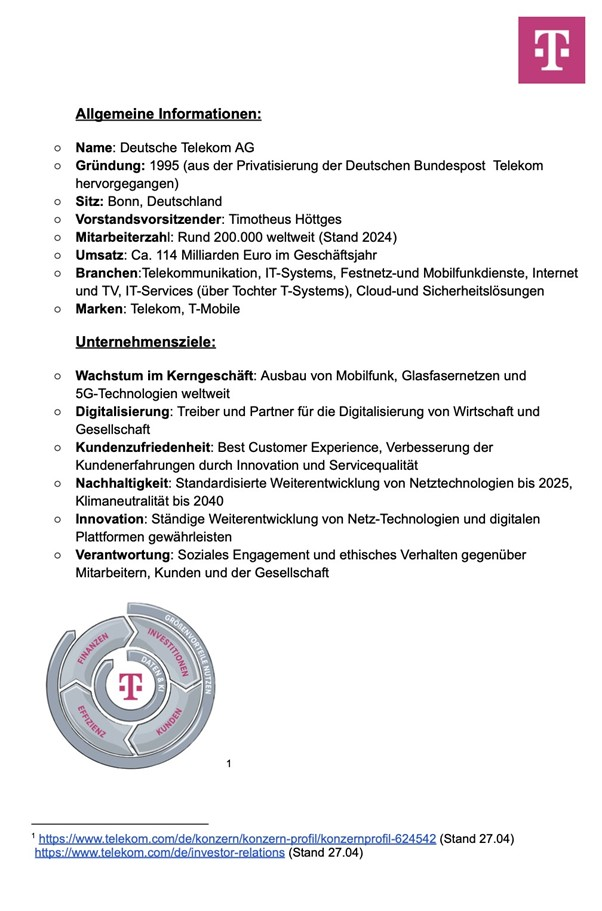
\includegraphics{images/Bild1.jpg}
	\end{figure}
	\newpage
	%------------------------- Anhang -------------------------
	\newpage
	\section{Anhang}
	[Zusätzliche Materialien wie Interviewleitfäden etc.]
	
	%------------------------- KI-Nutzung -------------------------
	\newpage
	\section{Anhang: Nutzung von Künstlicher Intelligenz}
	\begin{itemize}
		\item \textbf{Tool:} ChatGPT
		\item \textbf{URL:} \url{https://chatgpt.com}
		\item \textbf{Prompt:} „Erstelle eine vollständige LaTeX-Vorlage für eine Gruppenarbeit.“
		\item \textbf{Verwendet durch:} Mika Scheinig, Elija Wendte, Justus Kressmann, Engin Fidansoy, Manar Krenbeh
		\item \textbf{Datum:} 04.07.2025
	\end{itemize}
	\begin{itemize}
		\item \textbf{URL:} \url{https://chatgpt.com/share/682f2a68-37b8-8007-9855-d878bcd54ae3}
		\item \textbf{Prompt:} „Kannst du mir ein konkretes Beispiel für einen überregulierten internen Prozess der Deutschen Telekom nennen?“
		\item \textbf{Verwendet durch:} Mika Scheinig
		\item \textbf{Datum:} 22.05.2025
	\end{itemize}
	
	\begin{itemize}
		\item \textbf{URL:} \url{https://chatgpt.com/c/683721e2-4a9c-8001-b0a1-f2e5a1b3f5f2}
		\item \textbf{Prompt:} „Bitte erläutere die Unterschiede in der Leitungsspanne zwischen standardisierten operativen Bereichen und komplexeren Organisationseinheiten wie der Matrixorganisation bei T-Systems. Wie beeinflusst die Organisationsstruktur die Anzahl der direkt unterstellten Mitarbeitenden, und welche Herausforderungen ergeben sich für Führungskräfte in einer Matrixstruktur?“
		\item \textbf{Verwendet durch:} Justus Kressmann
		\item \textbf{Datum:} 24.05.2025
	\end{itemize}
	
	\newpage
	\section*{Eidesstattliche Erklärung}
	Hiermit versichern wir, dass wir die vorliegende Arbeit selbstständig und nur mit den angegebenen Hilfsmitteln und Quellen angefertigt haben. Alle Stellen, die wörtlich oder sinngemäß aus Quellen übernommen wurden, sind entsprechend kenntlich gemacht. Die Arbeit wurde in gemeinsamer Verantwortung erstellt.
	
	\vspace{2cm}
	Oldenburg, 01. Juni 2025
	
	Unterschriften: \\
	\rule{5cm}{0.4pt} Mika Scheinig \\
	\rule{5cm}{0.4pt} Elija Wendte \\
	\rule{5cm}{0.4pt} Justus Kressmann \\
	\rule{5cm}{0.4pt} Engin Fidansoy \\
	\rule{5cm}{0.4pt} Manar Krenbeh
	
	
	
\end{document}
